\documentclass[11pt]{article}

% Change "review" to "final" to generate the final (sometimes called camera-ready) version.
% Change to "preprint" to generate a non-anonymous version with page numbers.
\usepackage[review]{acl}

% Standard package includes
\usepackage{times}
\usepackage{latexsym}

% For proper rendering and hyphenation of words containing Latin characters (including in bib files)
\usepackage[T1]{fontenc}
% For Vietnamese characters
% \usepackage[T5]{fontenc}
% See https://www.latex-project.org/help/documentation/encguide.pdf for other character sets

% This assumes your files are encoded as UTF8
\usepackage[utf8]{inputenc}

% This is not strictly necessary, and may be commented out,
% but it will improve the layout of the manuscript,
% and will typically save some space.
\usepackage{microtype}

% This is also not strictly necessary, and may be commented out.
% However, it will improve the aesthetics of text in
% the typewriter font.
% Commented out: inconsolata.sty is not available in this environment's TeX install.
% \usepackage{inconsolata}

%Including images in your LaTeX document requires adding
%additional package(s)
\usepackage{graphicx}

% If the title and author information does not fit in the area allocated, uncomment the following
%
%\setlength\titlebox{<dim>}
%
% and set <dim> to something 5cm or larger.

% \usepackage[margin=1in]{geometry}
\usepackage{booktabs}
\usepackage{multirow}
\usepackage{amsmath}
\usepackage{natbib}
\usepackage{xcolor}
\usepackage{tikz}
\usepackage{pgfplots}
\pgfplotsset{compat=1.17}
\usepgfplotslibrary{groupplots}

% Drafting conventions (retained from the original skeleton):
%  - \todo{...} = a decision or number still needed. None should remain at submission time.
%  - Single-table constraint: tab:main-results is the ONLY table in the paper.
%    All ablation/analysis numbers go into prose deltas or figures.
\newcommand{\todo}[1]{\textcolor{red}{[TODO: #1]}}
\newcommand{\method}{SCOTECI}

\title{\method{}: Synthetic Chain-of-Thought Demonstrations for Document-Level Event Causality Identification}
\author{}
\date{}

\begin{document}

\maketitle

% ======================================================================
\begin{abstract}
Large language models (LLMs) applied to Event Causality Identification (ECI) exhibit
\emph{causal hallucination}: near-total recall paired with unusable precision
\citep{gao2023chatgpt}. Prior LLM-based scaffolds for ECI, such as Dr.ECI and SERE,
fight this at the \emph{pair} level, issuing one call per candidate event pair with
bare input-to-label demonstrations \citep{cai2025dreci, hao2026sere}. We propose
\method{}, which instead (i) reformulates LLM-based ECI at the \emph{document} level,
labelling every pair of a document jointly in a single call under a structured
reasoning protocol with explicit coherence rules, and (ii) equips its few-shot
demonstrations with \emph{synthetic chain-of-thought}: gold-guided reasoning generated
by an LLM and then decontaminated so it reads as genuine discovery rather than answer
confirmation. The method needs no fine-tuning, no human-written rationales, and no
external knowledge base. On Causal-TimeBank, \method{} reaches F1 48.1 (precision
61.1) against F1 20.0 for the best prior LLM method --- a +28.1 F1 gain obtained by
breaking out of the degenerate high-recall/low-precision regime rather than trading
recall for precision, on the dataset where positives are sparsest and hallucination is
costliest. It also attains the best precision on MAVEN-ERE (40.8) and matches SERE's
F1 on EventStoryLine (51.7 vs.\ 49.9). Beyond the headline numbers, we present an
evidence-driven analysis of the method itself: majority-vote aggregation over
demonstration ensembles is empirically F1-optimal, precision \emph{rises} rather than
falls with document causal density, and synthetic chain-of-thought demonstrations help
chat-tuned backbones but measurably hurt a reasoning-tuned one.
\end{abstract}

% ======================================================================
\section{Introduction}
\label{sec:intro}

Event Causality Identification (ECI) asks, given a document and its marked event
mentions, whether a directed causal relation holds between each pair of events
\citep{cheng2025survey}. It is a building block for event forecasting, causal
question answering, and narrative and discourse understanding, and has been pursued
along two largely disjoint paths: fine-tuned encoders and, more recently, prompted
LLMs. Fine-tuned encoders --- BERT/RoBERTa-era models augmented with event-relational
graphs or external knowledge --- are strong in-domain but require per-corpus
annotation and generalize poorly outside the corpus they were trained on
\citep{cai2025dreci, hao2026sere}. Prompted LLMs sidestep the annotation cost
entirely, but exhibit \emph{causal hallucination}: on Causal-TimeBank, a plain
zero-shot or chain-of-thought prompt reaches 80--96\% recall with precision below
10\% (Table~\ref{tab:main-results}, Base/CoT rows) --- the model asserts a causal
link almost anywhere a temporal or narrative connection exists \citep{gao2023chatgpt}.

The LLM scaffolds designed to fix this --- Dr.ECI's four-agent discovery/reasoning
pipeline \citep{cai2025dreci}, SERE's structurally retrieved demonstrations over
ConceptNet paths and syntax-tree edit distance \citep{hao2026sere}, and DICP's
learned deep in-context prompts \citep{mu2025dicp} --- all operate at the
\emph{pair} level: one LLM call per candidate event pair, re-paying the full
document context every time. This has three consequences. First, cost scales as
$O(|\text{pairs}|)$ calls per document ($O(n^2)$ in the number of mentions), each
of which resends the whole document. Second, each pair is judged in isolation, so
nothing enforces symmetry or transitivity across the pairs of the same document, and
the model never sees the document's causal structure as a whole. Third, these
scaffolds were engineered around the specific weaknesses of 2023--2024-era models;
as base models improve, the scaffold increasingly caps rather than unlocks their
capability.

We propose \method{}, built on two ideas that invert this design. The first is to
operate at the \emph{document} level: a single call labels every pair of a document
jointly, guided by an in-prompt reasoning protocol (mention pre-filter $\to$
per-pair arguments for and against $\to$ plausibility ranking $\to$ final JSON)
together with explicit coherence rules --- symmetry and dataset-specific transitivity
--- that are checkable only because the whole graph is produced at once. This shifts
the burden of consistency from external orchestration to the model's own long-context
reasoning, which is a deliberate bet: the method should get better, not merely
cheaper, as the underlying model improves.

The second idea addresses what document-level demonstrations should look like. Bare
input$\to$gold-JSON demonstrations teach the model the output format but not how to
reason about it, and document-level human-written rationales for ECI do not exist
and would be expensive to produce. Since gold labels for training documents
\emph{are} available, we generate the reasoning instead: a demonstration document is
shown to an LLM together with its own task prompt and its gold labels, and the model
is asked to write reasoning that leads naturally to those labels (\emph{gold-guided
generation}); the response is then rewritten from scratch to remove any phrasing that
betrays foreknowledge of the answer (\emph{decontamination}), so that every sentence
reads as discovery rather than confirmation. An optional three-step variant inserts a
blind attempt before the gold-guided pass, preserving more of the texture of a
genuine, imperfect first try. Each demonstration becomes a (user, assistant) exchange
in the prompt, so the model effectively ``remembers having solved'' a handful of
documents correctly, reasoning included.

On Causal-TimeBank, \method{} reaches F1 48.1 (precision 61.1, recall 39.6) against
F1 20.0 for the best prior LLM method (SERE) --- a +28.1 F1 gain, with precision more
than four times any LLM baseline in the comparison (Table~\ref{tab:main-results}).
This is the dataset where positives are sparsest and hallucination is most punishing,
and it is also the dataset where the balanced precision/recall regime most clearly
replaces the degenerate high-recall/near-zero-precision one that every baseline
exhibits. \method{} additionally attains the best precision on MAVEN-ERE (40.8) and
an F1 that edges out SERE on EventStoryLine (51.7 vs.\ 49.9). All three \method{}
numbers are reported on the intra-sentence subset of pairs, which is the only subset
SERE itself evaluates, so this is the fair like-for-like comparison; full-document
(intra- and inter-sentence) prediction is a capability the document-level
formulation affords --- one call covers all pairs regardless of how many of them
cross a sentence boundary, whereas a pair-level method pays for every additional
inter-sentence pair as another call --- but is not yet measured for \method{} and is
left to future work (see Limitations).

Beyond the headline table, we use \method{}'s logged predictions to answer questions
the original design left open. We show that the majority-vote aggregation used
across resampled passes is empirically F1-optimal rather than merely
``precision-preserving'' as assumed, that precision \emph{rises} rather than falls
with a document's causal density --- the opposite of the attention-dilution failure
mode we originally expected --- and that synthetic chain-of-thought demonstrations
help chat-tuned backbones but measurably hurt a reasoning-tuned one, a finding with
direct implications for which future backbones the method should target.

Our contributions are:
\begin{itemize}
  \item A document-level reformulation of LLM-based ECI, with a structured in-prompt
        reasoning protocol and explicit coherence rules, that issues $O(1)$ LLM
        calls per document instead of $O(|\text{pairs}|)$ and produces predictions
        that are consistent across a document's pairs by construction.
  \item A synthetic chain-of-thought demonstration pipeline --- gold-guided
        generation followed by decontamination --- that is model-agnostic and needs
        no human-written rationales or external knowledge base.
  \item State-of-the-art LLM results on Causal-TimeBank by a wide margin, with
        balanced precision/recall on all three evaluated datasets, plus an
        evidence-based analysis of aggregation, document density, backbone
        interaction, cost, and robustness that goes beyond the headline comparison.
\end{itemize}

% ======================================================================
\section{Related Work}
\label{sec:related}


\subsection{Supervised and Knowledge-Enhanced ECI}
Before LLM prompting, ECI was dominated by fine-tuned encoders that inject
structural or external signal into a BERT/RoBERTa-style backbone: event-relational
graph transformers that propagate information across a document's mention graph
\citep{chen2022ergo}, sparse event representations for discriminative document-level
event-relation extraction \citep{yuan2023sendir}, joint identify-while-learn
objectives that couple mention and relation supervision \citep{liu2024ilif},
knowledge-guided binary question-answering formulations of the pairwise decision
\citep{wang2024knowqa}, and heterogeneous graph contrastive transfer for zero-shot
cross-lingual ECI \citep{he2024gimc}. These remain the strongest in-domain systems on
their respective benchmarks, but each requires gold-annotated training data for the
specific corpus (often the specific label scheme) it is evaluated on, and transfer
across corpora or languages is itself an active research problem rather than a given
\citep{he2024gimc}. \method{} requires no task-specific training at all: the
training split is used only as a pool of few-shot demonstrations.

\subsection{LLM-based ECI}
\citet{gao2023chatgpt} first showed systematically that ChatGPT-class models
over-predict causal links --- causal hallucination --- and established the
preprocessing and evaluation protocol that we and our baselines follow. Two
scaffolds subsequently targeted this failure mode at the pair level. Dr.ECI
decomposes each candidate pair into a discovery stage (a Causal Explorer and a
Mediator Detector) and a reasoning stage (Direct and Indirect Reasoners), guided by
causal-pattern DAG priors \citep{cai2025dreci}. SERE retrieves structurally similar
pair-level examples using ConceptNet shortest-path edit distance, dependency-tree
edit distance, and causal-pattern filtering, and balances positive and negative
demonstrations by construction \citep{hao2026sere}. Closer to our synthetic-rationale
idea, \citet{wang2024synthetic} frame ECI through a synthetic-control,
counterfactual-estimation lens, and DICP learns deep in-context prompts per pair
rather than retrieving them \citep{mu2025dicp}. All four of these methods (i)
prompt once per pair and (ii) show label-only demonstrations.

Two very recent methods are closer still to specific pieces of our design. Like
\method{}, CogECI operates at the document level and uses an LLM to produce
reasoning-adjacent signal --- grounded context pseudo-labels extracted from the
document --- but consumes that signal as supervision for a separately trained
graph network (a Sentence Graph Module and a Dual-Stream Causality Reasoning
Module) rather than as an in-context demonstration, so it remains a fine-tuned
method with an LLM-assisted labelling step, not a training-free prompting method
\citep{zhang2026cogeci}. \citet{zhao2026cottraces} generate chain-of-thought
traces specifically to reduce causal hallucination in ECI, the same failure mode
we target, but their traces are training data --- used to fine-tune small
($\leq$1.5B-parameter) models against a dedicated causal-hallucination-rate metric
--- rather than in-context demonstrations for a frozen, larger model, and their
unit of generation is a single relation rather than a whole document. \method{}
differs from all of the above on both axes at once: it prompts once per document
rather than once per pair or per relation, it shows demonstrations that carry
explicit reasoning rather than labels or pseudo-labels, and it requires no
fine-tuning whatsoever.

\subsection{In-Context Learning and Synthetic Rationales}
Chain-of-thought prompting improves multi-step reasoning by asking a model to
externalize intermediate steps before its final answer \citep{wei2022chain},
building on the broader observation that large models are effective few-shot
learners given the right demonstrations \citep{brown2020language}. In-context
learning, however, is highly sensitive to which demonstrations are shown and how
they are phrased \citep{liu2022makes, min2022rethinking}. Where rationales are not
naturally available, prior work has synthesized them: Auto-CoT clusters queries and
applies zero-shot CoT to generate rationales for demonstration selection
\citep{zhang2023autocot}; STaR bootstraps rationales through
\emph{rationalization} --- generating reasoning conditioned on a known answer ---
but consumes the result as fine-tuning data \citep{zelikman2022star}; step-by-step
distillation similarly extracts rationales as a training signal for smaller student
models \citep{hsieh2023distilling}. \method{} uses the same rationalization trick as
STaR, but differently: the synthesized reasoning is consumed \emph{at inference
time} as in-context demonstrations rather than as fine-tuning data, it operates at
document rather than sentence/example scale, and it adds an explicit decontamination
pass to strip answer-leakage phrasing --- without which, we find, demonstrations
teach the model to assert conclusions rather than to reason toward them
(\S\ref{sec:ablations}).

% ======================================================================
\section{Task Formulation}
\label{sec:task}

Given a document $D$ with event mentions marked inline in \texttt{<ID word>}
format, $M = \{m_1, \dots, m_n\}$, and a candidate pair set $P$ --- the annotated
pair list for corpora that provide one (the \emph{constrained} setting, used for
MECI and Causal-TimeBank) or all unordered mention pairs otherwise (the
\emph{open-ended} setting, used for MAVEN-ERE and EventStoryLine) --- the task is to
produce a complete labelling $\ell: P \to \{\textit{causes}, \textit{causedby},
\textit{norel}\}$: a unified, directed three-way label space into which every
corpus' native annotation scheme is mapped before evaluation. Concretely: MECI's
\textsc{CauseEffect}/\textsc{EffectCause}/\textsc{NoRel} labels map one-to-one onto
\textit{causes}/\textit{causedby}/\textit{norel}; MAVEN-ERE's \textsc{CAUSE} and
\textsc{PRECONDITION} relation types are both collapsed onto the same directed
causes/causedby pair; EventStoryLine's \textsc{PRECONDITION} and
\textsc{FALLING\_ACTION} relations are collapsed the same way; and Causal-TimeBank's
CLINK annotations map directly, restricted to the intra-sentence subset (286 of 318
CLINKs, 90\%; the remaining cross-sentence CLINKs are dropped at preprocessing, so
Causal-TimeBank has no genuine inter-sentence positives and consequently no
intra/inter split anywhere in this paper). For MAVEN-ERE, EventStoryLine, and
Causal-TimeBank, \textit{norel} pairs are not separately annotated in the source
data; they are the complement of the positive pairs within $P$.

Document-level inference means the model produces $\ell$ for \emph{all} of $P$ in a
single generation, formatted as a JSON array, in contrast to pair-level inference,
which issues $|P|$ independent queries, one per candidate pair.

We follow \citet{gao2023chatgpt}'s preprocessing and evaluation protocol for
comparability with \citet{hao2026sere} and \citet{cai2025dreci}: micro
precision/recall/F1 over the positive (causal) classes, \textit{norel} excluded from
the denominator, reported on the intra-sentence subset where a corpus distinguishes
intra- from inter-sentence pairs --- the subset SERE itself evaluates, and hence the
fair comparison point. We additionally adopt a binary framing throughout: once a
pair is identified as causal, whether it is scored as \textit{causes} or
\textit{causedby} is collapsed into a single positive class before computing
metrics, since the object of interest in this work is \emph{whether} a causal link
exists, not which of the two mentions is cause versus effect. Directed
(non-collapsed) metrics are logged for every run but are not the primary quantity we
report or optimize for.

% ======================================================================
\section{Method}
\label{sec:method}

\subsection{Overview}
The pipeline (Figure~\ref{fig:overview}) proceeds in four stages for each test
document: retrieve $k=3$ neighbour training documents (\S\ref{sec:retrieval});
generate and cache a synthetic chain-of-thought demonstration for each neighbour
(\S\ref{sec:synthcot}); assemble a multi-turn prompt in which every demonstration
appears as a past (user, assistant) exchange, followed by the test document; and
issue a single document-level call, under the structured reasoning protocol of
\S\ref{sec:docprompt}, whose parsed JSON output is optionally aggregated across $N$
resampled passes (\S\ref{sec:inference}). Two components carry the paper's
contribution --- the document-level structured prompt (\S\ref{sec:docprompt}) and
the synthetic chain-of-thought demonstrations (\S\ref{sec:synthcot}); neighbour
retrieval (\S\ref{sec:retrieval}) and aggregation (\S\ref{sec:inference}) are
deliberately kept simple, and \S\ref{sec:ablations} measures what each of the four
pieces contributes.

\begin{figure}[t]
  \centering
  \begin{tikzpicture}[
      node distance=4mm and 4mm,
      box/.style={draw, rounded corners, align=center, font=\scriptsize,
        minimum height=9mm, text width=15mm, fill=gray!8},
      arr/.style={->, thick}
    ]
    \node[box] (doc) {Test\\document};
    \node[box, right=of doc] (retrieve) {Retrieve\\$k{=}3$\\neighbours};
    \node[box, right=of retrieve] (cot) {Synthesize\\CoT\\(cached)};
    \node[box, below=8mm of cot] (assemble) {Assemble\\multi-turn\\prompt};
    \node[box, left=of assemble] (call) {Doc-level\\LLM call\\$\times N{=}3$};
    \node[box, left=of call] (vote) {Majority\\vote};
    \draw[arr] (doc) -- (retrieve);
    \draw[arr] (retrieve) -- (cot);
    \draw[arr] (cot) -- (assemble);
    \draw[arr] (assemble) -- (call);
    \draw[arr] (call) -- (vote);
  \end{tikzpicture}
  \caption{Overview of \method{}: neighbour retrieval (\S\ref{sec:retrieval}),
  synthetic CoT generation (\S\ref{sec:synthcot}), multi-turn prompt assembly and
  a single document-level call (\S\ref{sec:docprompt}), and majority-vote
  aggregation across $N$ resampled passes (\S\ref{sec:inference}).}
  \label{fig:overview}
\end{figure}

\subsection{Document-Level Structured Prompting}
\label{sec:docprompt}
One call handles the entire document: every pair in $P$ is requested at once, and
the model sees the full narrative rather than a windowed snippet around a single
pair. The system prompt enforces an in-prompt reasoning protocol with four ordered
steps. First, a mention-level pre-filter excludes mentions only via an
affirmatively argued reason (e.g., ``$m$ is a location with no agentive role''),
never a blanket dismissal, and lists which mentions survive. Second, for every
retained pair the model lays out arguments \emph{for} a causal link (an explicit
connective, a plausible mechanism, counterfactual asymmetry, supporting discourse
structure) and arguments \emph{against} it (a merely temporal relation, a
confounding third event, a reporting verb, excessive distance). Third, the
surviving pairs are ranked qualitatively by causal plausibility, without committing
to labels yet. Fourth, the model emits a final JSON labelling of \emph{every}
requested pair; anything excluded in step one defaults to \textit{norel}.

A precision-first rule block targets causal hallucination directly: a two-signal
requirement for non-overt links (at least two independent pieces of textual
evidence, not one), a stricter evidentiary gate for inter-sentential or otherwise
long-range pairs, a default to \textit{norel} under genuine uncertainty, an
explicit confounder/proximal-cause check, a rule that reporting and purely temporal
connectives are non-causal on their own, and a counterfactual direction test. One
dataset-specific instance of this rule block matters enough to disclose explicitly:
on Causal-TimeBank, the active prompt additionally requires an \emph{explicit
causal marker} directly connecting the two events for a \textit{causes}/
\textit{causedby} label, defaulting to \textit{norel} when no such marker is
present. Causal-TimeBank's CLINK annotation is itself markedly explicit-connective
(roughly half of gold links carry an overt causal marker), so the rule is
dataset-appropriate rather than a silent addition to ``the protocol''; a matched
ablation on the reported backbone (\S\ref{sec:ablations}) measures its isolated
contribution at +10 to +19 F1 out of the +28.1 F1 headline gain over SERE, and we
state the rule here rather than folding it into the generic rule block above.

Finally, the prompt states two coherence rules that are checkable only because the
whole pair set is produced jointly: symmetry
($\textit{causes}(i,j) \Leftrightarrow \textit{causedby}(j,i)$) and
dataset-specific transitivity rules (e.g.\ chains of MAVEN-ERE's
\textsc{PRECONDITION} relation compose transitively; full rule sets are provided
with the released configuration). In the runs behind Table~\ref{tab:main-results}
these rules are stated in-prompt only --- the pipeline also supports a post-hoc
tool that could mechanically check or prune violations after generation, but that
tool was disabled (\texttt{enable\_tools=False}) throughout, so their effect here
is whatever the model achieves by reading the rules, not by external enforcement;
\S\ref{sec:ablations} discusses why we cannot yet isolate their contribution from
the rest of the protocol.

This design leverages better models on purpose: the protocol asks for exactly the
kind of global, long-context reasoning that frontier models are differentially good
at, whereas pair-level scaffolds cap that ability at the width of a single pair.

\subsection{Neighbour-Document Retrieval}
\label{sec:retrieval}
The demonstration pool is the training split of the same corpus, capped to 100
documents (\texttt{pool\_size}) to bound the cost of synthetic CoT generation
(\S\ref{sec:synthcot}): every demonstration document needs its reasoning generated
once, so a larger pool means more one-off generation cost, amortized by caching
across the run but not free. Table~\ref{tab:main-results}'s \method{} row uses
\emph{random} selection: $k=3$ demonstrations sampled uniformly from the pool for
each call. We also implement three retrieval-based alternatives: TF-IDF cosine
similarity over the full document text, sentence-embedding cosine similarity, and
Jaccard similarity over the set of event-mention strings; the first two are
compared against random selection in \S\ref{sec:ablations}, while mention-set
Jaccard is implemented but has not yet been evaluated in any run. Every
demonstration is a \emph{whole document with its complete gold labelling},
including its \textit{norel} pairs, so each demonstration carries explicit negative
evidence for free --- the pair-level analogue of which SERE must engineer by
explicitly balancing positive and negative retrieved examples.

\subsection{Synthetic Chain-of-Thought Generation}
\label{sec:synthcot}
Label-only demonstrations teach the output schema but not the reasoning behind it;
document-level human rationales are unavailable and would be prohibitively
expensive to write; but gold labels for training documents \emph{are} available, so
rationales can be synthesized instead. In the default 2-step protocol, each
demonstration document is (i) shown under the exact task prompt together with its
gold labels, with an instruction to write reasoning that ``leads naturally to these
labels from the text alone'' without revealing foreknowledge (\emph{gold-guided
generation}), and then (ii) rewritten from scratch to purge leakage phrasing
(``the labels show\dots'', ``as indicated by the expected output\dots''), so every
sentence reads as analysis rather than confirmation (\emph{decontamination}). A
3-step variant inserts a blind attempt with no gold access before the gold-guided
correction step, so the sequence becomes blind attempt $\to$ gold-based correction
(fixing wrong conclusions while keeping correct reasoning) $\to$ decontamination;
this preserves more of the texture and difficulty profile of a genuine, imperfect
first try. Table~\ref{tab:main-results}'s \method{} row uses the 3-step variant; a
limited 2- vs.\ 3-step comparison exists (\S\ref{sec:ablations}), but the
difference falls within run-to-run noise on the runs available so far.

Each demonstration becomes a (user task turn, assistant CoT turn) exchange
preceding the test document, so the model effectively ``remembers having done'' $k$
documents correctly, reasoning included; this is compatible with multi-step task
prompts, which receive one synthetic response per step. Demonstrations are
generated once per (document, protocol) and cached for the remainder of the run;
unless noted otherwise, the generator model is the same as the inference model
(self-generated rationales) --- whether a stronger generator can lift a weaker
reasoner is a question we leave open (see Limitations). Decontamination is not
currently an optional step: both the 2- and 3-step protocols apply it
unconditionally, so while we motivate it as necessary (\S\ref{sec:related}), we do
not yet have a controlled ablation that isolates its effect from a
from-scratch demonstration generated without it; \S\ref{sec:ablations} reports
what the current logs can and cannot support on this point.

The relation to STaR-style rationalization \citep{zelikman2022star} is direct: the
same trick --- condition on the answer to obtain reasoning --- but used as
in-context demonstrations at inference time rather than as fine-tuning data, and
with an explicit decontamination pass that we motivate as necessary for the
demonstrations to teach reasoning rather than assertion.

\subsection{Inference and Aggregation}
\label{sec:inference}
Decoding uses temperature 0 with strict JSON parsing and bounded retries; a
document that exhausts all retries is scored as entirely \textit{norel} rather than
excluded from evaluation (2 of 183 Causal-TimeBank documents fall into this
category for the headline run; EventStoryLine and MAVEN-ERE have none). Pairs
absent from a parsed response also default to \textit{norel}.

Table~\ref{tab:main-results}'s \method{} row uses $N=3$ resampling passes per
document with a per-pair majority vote, ties broken to \textit{norel}; each pass
draws its own set of $k$ demonstrations independently
(\texttt{distinct\_fewshots=True}), split round-robin from a larger draw so the
three passes' demonstration sets are disjoint. We originally intended pair-order
reshuffling across passes to be the source of inter-pass disagreement, but at
temperature 0, and with the candidate pair list identical across passes for the
constrained-pair-list datasets, reshuffling has no effect once the pair list itself
does not change. What actually differs between passes is \emph{which}
demonstrations they see. ``Resampling with majority vote'' is therefore better
understood as an ensemble over demonstration sets, plus whatever provider-level
nondeterminism survives temperature 0, rather than as stochastic resampling of an
otherwise-fixed call. \S\ref{sec:analysis} shows that this reframing explains why
passes disagree at all --- false positives are pass-specific while true positives
are stable across the ensemble --- and that the resulting majority-vote rule is
empirically F1-optimal on all three datasets, not merely precision-preserving by
assumption.

Cost per document is 1 call under \method{} ($N$ under resampling), plus the
amortized, cached cost of generating each demonstration's synthetic CoT once (2 or
3 extra calls per unique demonstration document, shared across every test document
that retrieves it). This contrasts with $|P|$ calls per document for pair-level
methods, each resending the document, plus SERE's per-pair retrieval
infrastructure (ConceptNet and a dependency parser) and Dr.ECI's up to four agent
calls per pair; \S\ref{sec:cost} quantifies the resulting gap using the tokens and
dollar costs logged for the headline runs.

% ======================================================================
\section{Experiments}
\label{sec:experiments}

\subsection{Datasets and Metrics}
We evaluate on three English ECI corpora spanning news and Wikipedia text, chosen
to vary substantially in positive-pair density and scale.

\textbf{EventStoryLine} (ESC; \citealp{caselli2017event}), version 0.9: 258 news
documents across 22 topics, with causal (\textsc{PRECONDITION}/
\textsc{FALLING\_ACTION}) links annotated over ECB+ event chains. Following the
corpus's original convention, documents in topics 37 and 41 are held out as a
development split; we evaluate on the remaining 233 documents (the \texttt{train}
split), with 5-fold separation ensuring a document's few-shot demonstrations never
come from its own fold.

\textbf{Causal-TimeBank} (CTB; \citealp{mirza2014annotating}): 183 news documents,
318 CLINK-annotated causal pairs, of which 286 (90\%) are intra-sentence
(\S\ref{sec:task}) --- the sparsest-positive of the three corpora and,
consequently, the one where causal hallucination is most costly. As with ESC, we
evaluate on the full corpus, with 10-fold demonstration separation.

\textbf{MAVEN-ERE} \citep{wang2022mavenere}: a large-scale Wikipedia corpus with
57{,}992 causal pairs (\textsc{CAUSE} and \textsc{PRECONDITION}, collapsed as in
\S\ref{sec:task}) across its full release. We evaluate on its 710-document test
split (33{,}144 candidate pairs), using the training split as the demonstration
pool.

All preprocessing and label mapping follows \citet{gao2023chatgpt}'s protocol
(\S\ref{sec:task}) for comparability with our baselines. We additionally have
exploratory results on MECI \citep{lai2022meci}, a multilingual ECI corpus the
pipeline fully supports; those results are noisy across repeated runs of the same
configuration and are not yet at the standard of the three corpora above, so we
omit them from the main comparison (see Limitations).

\subsection{Baselines}
We compare against the LLM-prompted methods surveyed in \S\ref{sec:related}:
\textbf{Base}, a task description with no reasoning scaffold; \textbf{CoT}
\citep{wei2022chain}, step-by-step reasoning before the final answer;
\textbf{Dr.ECI} \citep{cai2025dreci}; and \textbf{SERE} \citep{hao2026sere}. All
four are pair-level: one call per candidate pair. The GPT-4o-mini and
Gemini-1.5-pro rows are reproduced from \citet{hao2026sere}'s Table 2; the PaLM2
Dr.ECI row is reproduced from \citet{cai2025dreci}. We do not re-run any baseline
ourselves, so differences between \method{} and these rows reflect both the
document-level reformulation and a different backbone; we do not yet have a
same-backbone pair-level control that would separate the two effects
(\S\ref{sec:cost} discusses why, and what evidence we have instead).

\subsection{Implementation Details}
Unless noted otherwise, \method{} uses \texttt{deepseek/deepseek-v4-pro} (via
OpenRouter) as both the inference and the CoT-generation backbone, at temperature
0. This is a mid-tier open model rather than a frontier one; \S\ref{sec:scaling}
reports what a limited, single-seed comparison across backbones (including a
frontier model) suggests about how the method scales with model quality, and
\S\ref{sec:cost} shows it is already competitive with a frontier backbone on a
cost-per-F1 basis. Demonstrations use $k=3$, random selection from a pool of 100
training documents, and the 3-step synthetic CoT protocol (\S\ref{sec:synthcot}).
The headline numbers use $N=3$ resampling passes with distinct demonstration sets
per pass and a majority vote (\S\ref{sec:inference}). Exact prompts (per dataset),
CoT-generation prompts, and coherence rule sets are versioned with the released
configuration.

Synthetic CoT generation costs 2 (2-step) or 3 (3-step) additional LLM calls per
unique demonstration document, amortized across every test document that draws it
from the shared pool. This cost is not separately metered in our logs but is
included in the total costs reported in \S\ref{sec:results} and \S\ref{sec:cost};
isolating it precisely would require either per-call cost tagging or mining token
counts from the cached CoT text, which we leave for future tooling.

\subsection{Main Results}
\label{sec:results}

% ----------------------------------------------------------------------
% Single merged results table.
% Baseline rows (PaLM2 / GPT-4o-mini / Gemini-1.5-pro blocks) are
% reproduced from SERE (Hao et al. 2026), Table 2. SERE itself evaluates
% intra-sentence pairs only, so SCOTECI's intra-sentence numbers (marked *)
% are the fair like-for-like comparison, not an incomplete one; CTB has no
% intra/inter split in the original data (all evaluated pairs are intra),
% so its column needs no asterisk. Full-document (intra+inter) SCOTECI
% numbers do not exist yet -- see the Limitations section.
% Bold = best score per column across the whole table (all rows).
% ----------------------------------------------------------------------
\begin{table*}
\begin{tabular}{l ccc|ccc|ccc}
\toprule
 & \multicolumn{3}{c|}{ESC} & \multicolumn{3}{c|}{CTB} & \multicolumn{3}{c}{MAVEN-ERE} \\
Method & P & R & F1 & P & R & F1 & P & R & F1 \\
\midrule
\textbf{PaLM2:} & & & & & & & & & \\
\quad Dr.ECI$^\dagger$ & 29.0 & 75.4 & 41.9 & - & - & 13.0 & 22.0 & 80.0 & 34.5 \\
\midrule
\textbf{GPT-4o-mini:} & & & & & & & & & \\
\quad Base          & 28.4 & 82.9 & 42.3 & 5.4  & 80.5 & 10.1 & 23.1 & 91.5 & 36.9 \\
\quad CoT           & 29.4 & 80.6 & 43.1 & 6.3  & 79.6 & 11.6 & 25.4 & 87.9 & 39.4 \\
\quad Dr.ECI        & 31.0 & \textbf{90.2} & 46.1 & 8.2  & 91.2 & 15.1 & 26.0 & 93.0 & 40.7 \\
\quad SERE          & \textbf{48.3} & 51.5 & \textbf{49.9} & 13.8 & 36.3 & 20.0 & 34.5 & 54.6 & \textbf{42.3} \\
\midrule
\textbf{Gemini-1.5-pro:} & & & & & & & & & \\
\quad Base          & 24.0 & 80.8 & 37.0 & 4.7  & \textbf{95.6} & 9.0  & 21.2 & \textbf{95.1} & 34.6 \\
\quad CoT           & 25.1 & 85.4 & 38.7 & 4.7  & 88.5 & 8.9  & 23.3 & 89.2 & 37.0 \\
\quad Dr.ECI        & 27.6 & 82.0 & 41.3 & 7.2  & 88.5 & 13.3 & 23.4 & 91.7 & 37.3 \\
\quad SERE          & 36.5 & 59.3 & 45.2 & 9.9  & 69.9 & 17.4 & 29.9 & 60.2 & 39.9 \\
\midrule
\textbf{Ours:} & & & & & & & & & \\
\quad SCOTECI$^*$   & 40.7 & 70.9 & 51.7 & \textbf{61.1} & 39.6 & \textbf{48.1} & \textbf{40.8} & 59.6 & 48.4 \\
\bottomrule
\end{tabular}
\centering
\small
\caption{Main results. Baseline rows reproduced from \citet{hao2026sere} (their Table 2). Best score per column is in bold across all rows. $\dagger$: results from \citet{cai2025dreci}. CTB has no intra/inter split, so its column is directly comparable throughout. On ESC and MAVEN-ERE, SERE itself evaluates intra-sentence pairs only, so SCOTECI's intra-sentence scores ($^*$) are the fair like-for-like comparison; full-document (intra+inter) SCOTECI numbers are additional future work (see Limitations), not a gap in this comparison.}
\label{tab:main-results}
\end{table*}

Table~\ref{tab:main-results} reports precision, recall, and F1 for \method{}
against the LLM baselines surveyed in \S\ref{sec:experiments}, all evaluated on the
intra-sentence subset (\S\ref{sec:task}).

\paragraph{Causal-TimeBank (the headline).} \method{} reaches F1 48.1 against 20.0
for the best LLM baseline (SERE) --- a +28.1 F1 gain --- with precision 61.1 where
no LLM baseline exceeds 13.8. This is the dataset with the sparsest positives and
the costliest hallucination, and it is where the degenerate high-recall/
low-precision regime is broken most clearly: every baseline sits at recall
$\ge$79.6 with precision $\le$13.8, while \method{} inverts the ratio entirely
(P 61.1, R 39.6). A matched ablation (\S\ref{sec:ablations}) measures roughly
+10 to +19 F1 of this gain as coming from a dataset-specific prompt rule rather
than from the document-level scaffold alone (\S\ref{sec:docprompt}); we report
that decomposition in full there rather than overstating what the scaffold alone
contributes here.

\paragraph{MAVEN-ERE.} \method{} attains the best precision in the table (40.8) and
an F1 of 48.4, exceeding SERE's 42.3 by 6.1 F1, on the full 710-document test split
(33{,}144 candidate pairs) --- making this the most heavily evaluated of the three
columns.

\paragraph{EventStoryLine.} \method{} reaches F1 51.7 (P 40.7, R 70.9), edging out
SERE's 49.9 while trading some of SERE's precision for recall. Unlike CTB and
MAVEN-ERE, \method{}'s precision on ESC (40.7) sits closer to the CoT/Dr.ECI
baseline range than to SERE's, so the gain here comes primarily from recall rather
than precision --- the opposite pattern from CTB.

\paragraph{Reading across rows.} Base, CoT, and Dr.ECI all sit at recall $\ge$75
with precision $\le$31 on every dataset, the hallucination signature described in
\S\ref{sec:intro}. SERE trades recall for precision but never exceeds P 48.3.
\method{} attains the best precision on two of three datasets (CTB, MAVEN-ERE) and
the best F1 on two of three (ESC, MAVEN-ERE), without ever collapsing into the
degenerate low-precision regime that Base/CoT/Dr.ECI exhibit everywhere.

\paragraph{On significance.} Each cell in \method{}'s row is a single
configuration's result (with $N=3$ resampling folded in, \S\ref{sec:inference}),
not a multi-seed mean. Repeated identical-configuration runs elsewhere in our logs
put the run-to-run standard deviation on 50-document subsets at roughly 2--4 F1
(ten repeats of one Causal-TimeBank configuration ranged 39.8--51.0 F1), and a
broader sweep of 31 byte-identical-configuration reruns has a median F1 spread of
0.02 and a 75th-percentile spread of 0.09 (0--1 scale). The Causal-TimeBank gain
over SERE (+28.1 F1) and the MAVEN-ERE gain (+6.1 F1) are both well outside this
noise band; the EventStoryLine gain (+1.8 F1) is not, and should be read as ``at
least competitive with,'' not ``reliably better than,'' SERE on that dataset.
\S\ref{sec:ablations} discusses what multi-seed reporting of the ablation deltas
would require.

% ======================================================================
\section{Analysis}
\label{sec:analysis}
% Single-table constraint: everything below reported as prose deltas
% ("removing X costs Y F1 on CTB") or as figures, never new tables.

\subsection{Ablations}
\label{sec:ablations}

Every ablation below is reported as a prose delta against a matched configuration
rather than as a new table, and calibrated against the noise floor established in
\S\ref{sec:results}: on 50-document subsets, run-to-run F1 standard deviation is
roughly 2--4, and a broader sweep of byte-identical reruns puts the median spread
at 0.02 and the 75th percentile at 0.09 (0--1 scale). Much of what is available
today is single-seed, on an earlier backbone, or otherwise confounded, and we
report that plainly rather than presenting underpowered comparisons as settled.

\textbf{Explicit-marker rule (Causal-TimeBank), on the final backbone.} Unlike the
ablations below, this one is a clean, matched, current-backbone comparison rather
than an inherited estimate: two matched pairs on \texttt{deepseek-v4-pro}
(Causal-TimeBank, $n$=50, $k$=3 random demonstrations, pool 20, 3-step CoT) ---
one pair with resampling off, one with $N$=3 resampling --- compare the
explicit-marker prompt (\S\ref{sec:docprompt}) against an otherwise-identical
prompt with the marker requirement removed. Without resampling: marker F1 39.6
vs.\ no-marker 21.0, a +18.6 F1 gain. With $N$=3 resampling: marker F1 47.5 vs.\
no-marker 37.2, a +10.3 F1 gain. Both deltas are well outside the noise floor and
confirm, on the actual reported backbone, what the earlier v3.2-era decomposition
only suggested: the marker rule does substantial, real work, though on
\texttt{deepseek-v4-pro} its isolated contribution (+10 to +19 F1) is smaller than
the roughly +30 F1 estimated on the older backbone --- consistent with a stronger
backbone needing the explicit hint less. This closes the gap the ablation audit
behind this section originally flagged as missing.

\textbf{Synthetic CoT vs.\ label-only demonstrations.} On the Causal-TimeBank
explicit-marker prompt, matched runs on an earlier backbone (\texttt{deepseek-v3.2})
put CoT demonstrations at F1 43.1 (mean of 13 runs) against 34.1 for label-only
demonstrations (a single run), a +9.0 F1 gain. We do not yet have a matched
comparison on the final \texttt{deepseek-v4-pro} configuration, and
\S\ref{sec:cotbackbone} reports a complicating finding: the same substitution
\emph{hurts} a reasoning-tuned backbone by a comparable margin, so whether CoT
demonstrations help is backbone-dependent rather than uniformly true.

\textbf{Few-shot on/off and protocol on/off.} An early-backbone Causal-TimeBank run
with few-shot disabled entirely scored F1 40.9, \emph{above} the label-only-demo
condition above (34.1) on a single seed each --- suggestive that badly-chosen
demonstrations can cost more than they give, but not a clean result. Removing the
structured protocol (the \texttt{*\_norule*} prompt variants, demonstrations kept)
shows small, noise-level differences on EventStoryLine (41.4 vs.\ 40.8--44.4) and
MAVEN-ERE (33.6 vs.\ 34.8--36.6, earlier backbone); Causal-TimeBank's only
no-protocol runs predate the explicit-marker rule and are not comparable. Neither
comparison currently supports a quantitative claim about the structured protocol's
contribution in isolation.

\textbf{Demonstration selection.} Random selection matches or exceeds TF-IDF and
sentence-embedding retrieval at document scale: on MAVEN-ERE (matched setting,
\texttt{deepseek-v4-pro}), random selection scores 45.0--47.1 F1 across four runs,
embedding retrieval 37.5--46.6 across eight runs, and TF-IDF 39.6 on a single run.
This echoes, at document scale, SERE's own report that naive retrieval can
underperform random selection at pair level \citep{hao2026sere}, and matches our
choice of random selection for the headline table (\S\ref{sec:retrieval}).
Mention-Jaccard selection is implemented but has not yet been run. A related
trend: larger demonstration pools (more per-document diversity to sample from)
trend positive, though not for free --- diverse per-document demonstrations reduce
prompt-cache reuse, and our headline runs read only 18--21\% of input tokens from
cache; a fixed demonstration set would be materially cheaper to serve but likely
somewhat worse.

\textbf{Number of demonstrations.} All headline runs use $k=3$. A single MAVEN-ERE
comparison exists at $k=6$ (39.4 vs.\ 38.4 for matched $k=3$, both single runs);
$k=1$ and $k=5$ have not been run. We cannot yet say whether document-level
demonstrations saturate or degrade past $k=3$, as pair-level demonstrations do
past $k=2$ in SERE.

\textbf{2-step vs.\ 3-step CoT.} Two matched pairs exist: EventStoryLine (2-step
41.8 vs.\ 3-step 40.6) and MAVEN-ERE, earlier backbone (2-step 38.9 vs.\ 3-step
39.3). Both differences are within run-to-run noise. We use the 3-step variant for
the headline table on the strength of its intended benefit (preserving the texture
of a genuine attempt, \S\ref{sec:synthcot}) rather than a measured advantage.

\textbf{Decontamination on/off.} We motivate decontamination as necessary
(\S\ref{sec:synthcot}, \S\ref{sec:related}), but the current implementation applies
it unconditionally in both CoT protocols, so isolating its effect requires a
configuration option that does not yet exist; a raw, non-decontaminated variant
has been run only once, on a single document, as a smoke test. This ablation is
missing, not merely underpowered, and is the clearest concrete item of future work
this paper leaves (see Limitations).

\textbf{Coherence rules on/off.} The post-hoc coherence-checking tool was disabled
in every run behind Table~\ref{tab:main-results} (\S\ref{sec:docprompt}), so no
run isolates the in-prompt coherence rules from the rest of the protocol; earlier
tool-enabled runs use different prompts and models and are not comparable. This
ablation, like decontamination, is currently missing rather than inconclusive.

\subsection{Aggregation: Majority Vote Is Empirically F1-Optimal}
\label{sec:voting}

\S\ref{sec:inference} reframes resampling as an ensemble over demonstration sets
rather than stochastic resampling. This lets us ask directly whether the shipped
aggregation rule --- majority vote of $N=3$ passes, ties broken to \textit{norel}
--- is actually the best choice, by sweeping the vote threshold $t \in \{1,2,3\}$
(predict causal iff at least $t$ of the 3 passes agree) over the full per-pair
predictions of the three headline runs, reconstructed from their raw per-pass
traces.\footnote{Reconstructed rather than read from the logged per-pair
predictions, which for these runs retain only gold~$\cup$~final-majority pairs and
would silently hide exactly the pass-specific false positives a union rule adds;
the reconstruction reproduces each run's logged majority-vote metric within
0.1--1.1 F1, which we take as validating the reconstruction.} Figure~\ref{fig:vote}
plots precision, recall, and F1 at each threshold for all three datasets.

Majority voting ($t=2$) is F1-optimal on all three datasets: union voting ($t=1$)
costs 3.5--5.2 F1 relative to it, and unanimous voting ($t=3$) costs 0.8--3.0 F1.
The reason is asymmetric reliability: on Causal-TimeBank, 70\% of the false
positives that union voting adds appear in only one of the three passes, while
72\% of union's true positives survive into the majority --- per-pass
hallucinations are largely ephemeral, and the vote filters them out, while genuine
signal is stable across the demonstration ensemble. Unanimous voting is
nonetheless a real, usable precision mode for applications that need it
(Causal-TimeBank P 76.7, MAVEN-ERE P 49.0, EventStoryLine P 46.9), and union
recall (55.0 / 75.8 / 83.5) measures the recall ceiling of the demonstration
ensemble as a whole. Ties-to-\textit{norel} (\S\ref{sec:inference}) is therefore
not merely a reasonable default but the empirically correct one for our reported
configuration.

\begin{figure}[t]
  \centering
  \begin{tikzpicture}
  \begin{groupplot}[
      group style={group size=3 by 1, horizontal sep=3mm},
      ybar, bar width=3pt,
      width=0.31\linewidth, height=3.1cm,
      ymin=0, ymax=90,
      symbolic x coords={t=1,t=2,t=3},
      xtick=data,
      tick label style={font=\tiny},
      label style={font=\tiny},
      legend style={font=\tiny, at={(0.5,1.32)}, anchor=south, legend columns=3},
    ]
    \nextgroupplot[title={CTB}, title style={font=\scriptsize},
      ylabel={score}, ylabel style={font=\tiny}]
      \addplot coordinates {(t=1,36.1) (t=2,57.8) (t=3,76.7)};
      \addplot coordinates {(t=1,55.0) (t=2,39.6) (t=3,30.9)};
      \addplot coordinates {(t=1,43.6) (t=2,47.0) (t=3,44.0)};
      \legend{P,R,F1}
    \nextgroupplot[title={ESC}, title style={font=\scriptsize}]
      \addplot coordinates {(t=1,31.8) (t=2,40.1) (t=3,46.9)};
      \addplot coordinates {(t=1,83.5) (t=2,71.0) (t=3,54.5)};
      \addplot coordinates {(t=1,46.1) (t=2,51.3) (t=3,50.5)};
    \nextgroupplot[title={MAVEN-ERE}, title style={font=\scriptsize}]
      \addplot coordinates {(t=1,31.8) (t=2,40.5) (t=3,49.0)};
      \addplot coordinates {(t=1,75.8) (t=2,59.8) (t=3,41.7)};
      \addplot coordinates {(t=1,44.8) (t=2,48.3) (t=3,45.1)};
  \end{groupplot}
  \end{tikzpicture}
  \caption{Precision, recall, and F1 as a function of the resampling vote
  threshold $t$, on the three headline runs. Majority ($t{=}2$) is F1-optimal
  everywhere.}
  \label{fig:vote}
\end{figure}

\subsection{Document-Level vs.\ Pair-Level, Same Backbone}
\label{sec:cost}

The internal comparison that would most cleanly separate the document-level
formulation's effect from the choice of backbone --- the same model, forced into
one-call-per-pair inference under the same rules --- is not currently implemented
in our pipeline (\texttt{prompts/esl\_perpair.yaml} exists but was never run to
completion as a controlled comparison), and we do not have it to report. What we
do have is an arithmetic cost argument and a measured cost-effectiveness result.

On calls and tokens: a pair-level method issues $|P|$ calls per document, each
re-sending the full document; on MAVEN-ERE's evaluated split alone, $|P|=33{,}144$
against 710 single-call \method{} documents (plus $N=3$ resampling and the
amortized, cached cost of demonstration CoT generation). Dr.ECI additionally
issues up to four agent calls per pair \citep{cai2025dreci}, and SERE's per-pair
retrieval requires a ConceptNet lookup and a dependency parse for every candidate
pair \citep{hao2026sere}. Measured end-to-end costs for the three headline runs
(inference plus resampling plus CoT generation) are \$7.49 (Causal-TimeBank),
\$13.19 (EventStoryLine), and \$24.15 (MAVEN-ERE).

Separately, on the same MAVEN-ERE 50-document setting used for the model ladder
(\S\ref{sec:scaling}), our mid-tier backbone (\texttt{deepseek-v4-pro}) matches or
exceeds a frontier model (\texttt{gpt-5.5}: F1 40.1 at \$7.23) at F1 39.6--45.2 for
\$0.66--1.12 --- roughly an order of magnitude better cost-per-F1
(Figure~\ref{fig:cost}); \texttt{glm-5.2} reaches F1 40.4 at \$1.81 and
\texttt{gpt-4o-mini} reaches F1 24.3. This is a stronger, already-measured version
of the cost argument that a same-backbone pair-level control would have made:
\method{} on a mid-tier open backbone is both more accurate and, per unit of F1,
an order of magnitude cheaper than one plausible pair-level cost driver --- using
a frontier model to compensate for a weaker scaffold.

\begin{figure}[t]
  \centering
  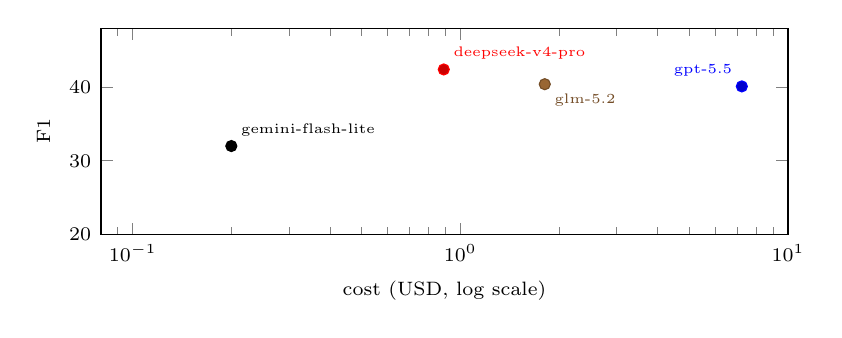
\begin{tikzpicture}
  \begin{axis}[
      width=0.85\linewidth, height=4.2cm,
      xmode=log,
      xlabel={cost (USD, log scale)}, ylabel={F1},
      label style={font=\scriptsize}, tick label style={font=\scriptsize},
      xmin=0.08, xmax=10, ymin=20, ymax=48,
      only marks,
    ]
    \addplot+[mark=*] coordinates {(7.23,40.1)}
      node[above left, font=\tiny] {gpt-5.5};
    \addplot+[mark=*] coordinates {(0.89,42.4)}
      node[above right, font=\tiny] {deepseek-v4-pro};
    \addplot+[mark=*] coordinates {(1.81,40.4)}
      node[below right, font=\tiny] {glm-5.2};
    \addplot+[mark=*] coordinates {(0.2,32.0)}
      node[above right, font=\tiny] {gemini-flash-lite};
  \end{axis}
  \end{tikzpicture}
  \caption{Cost-effectiveness: F1 vs.\ evaluation cost by backbone, MAVEN-ERE
  $n$=50 (single seed per point; deepseek-v4-pro and the gemini-flash-lite tier
  are plotted at the midpoint of their reported ranges).}
  \label{fig:cost}
\end{figure}

\subsection{Scaling with Model Quality}
\label{sec:scaling}

The claim we set out to test is that the document-level formulation's advantage
over pair-level prompting \emph{widens} as the backbone improves, because it
exposes rather than bypasses a model's long-context global reasoning. We do not
yet have the evidence to make that claim in its strongest (crossover) form: doing
so needs a pair-level arm at each point on a model ladder, and \S\ref{sec:cost}
explains why that arm does not exist yet. What we have instead is a single-seed,
partially confounded ladder of \method{} scores across backbones on MAVEN-ERE
(intra-sentence, $n=50$): \texttt{gpt-5.5} 40.1, \texttt{glm-5.2} 40.4,
\texttt{deepseek-v4-pro} 38.4--45.2 (varying with pool size and selection),
\texttt{deepseek-v3.2} 37.8--39.9, \texttt{qwen3-30b-thinking} 35.9,
\texttt{gemini-2.5-flash-lite} 34.0, \texttt{gemini-3.1-flash-lite} 30.1, and
\texttt{gpt-4o-mini} 24.3 (Figure~\ref{fig:ladder}). The direction is consistent
with ``bigger and more capable backbones score higher,'' and an isolated
Causal-TimeBank data point is suggestive in the expected direction --- with
few-shot disabled, \texttt{gpt-5.4-mini} collapses to 9.5 F1 where
\texttt{deepseek-v3.2} reaches 35.8 under the same configuration, consistent with
weaker models over-generating causal links at document scale --- but with every
point a single seed and no pair-level counterpart, we present this section as
evidence that \method{} \emph{improves with backbone quality}, not as evidence for
the specific doc-vs-pair crossover we originally hypothesized. \S\ref{sec:cost}'s
cost-effectiveness result is the more solid claim available today.

\begin{figure}[t]
  \centering
  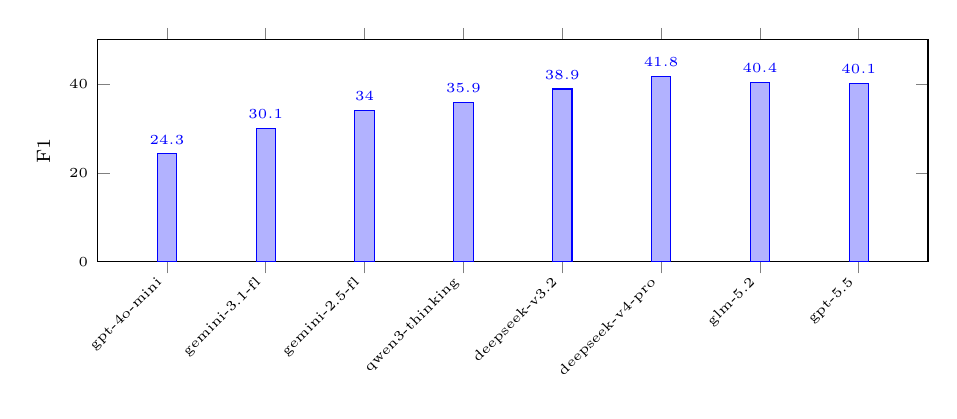
\begin{tikzpicture}
  \begin{axis}[
      ybar, bar width=7pt,
      width=\linewidth, height=4.4cm,
      ymin=0, ymax=50,
      symbolic x coords={gpt-4o-mini,gemini-3.1-fl,gemini-2.5-fl,qwen3-thinking,
        deepseek-v3.2,deepseek-v4-pro,glm-5.2,gpt-5.5},
      xtick=data,
      x tick label style={rotate=45, anchor=east, font=\tiny},
      tick label style={font=\tiny},
      ylabel={F1}, ylabel style={font=\scriptsize},
      nodes near coords, nodes near coords style={font=\tiny},
    ]
    \addplot coordinates {
      (gpt-4o-mini,24.3) (gemini-3.1-fl,30.1) (gemini-2.5-fl,34.0)
      (qwen3-thinking,35.9) (deepseek-v3.2,38.9) (deepseek-v4-pro,41.8)
      (glm-5.2,40.4) (gpt-5.5,40.1)
    };
  \end{axis}
  \end{tikzpicture}
  \caption{\method{} F1 across backbones, MAVEN-ERE intra, $n$=50, single seed
  per point (deepseek-v4-pro and deepseek-v3.2 shown at the midpoint of their
  reported ranges; x-axis ordered low-to-high by this measurement, not by a
  fixed independent tier ranking).}
  \label{fig:ladder}
\end{figure}

\subsection{Synthetic CoT Interacts with Backbone Reasoning Style}
\label{sec:cotbackbone}

A second, unplanned finding emerged from the CoT-on/off comparisons collected for
\S\ref{sec:ablations}: whether synthetic CoT demonstrations help depends on
whether the backbone has its own trained reasoning channel. Comparing matched
few-shot runs with CoT demonstrations against label-only demonstrations (same
dataset, model, and prompt), chat-tuned backbones benefit --- \texttt{deepseek-v3.2}
on Causal-TimeBank: +9.0 F1 (43.1 vs.\ 34.1, 13 vs.\ 1 runs); \texttt{glm-5.2} on
MECI: +16.2 (60.4 vs.\ 44.2, 1 run each) --- while the reasoning-tuned
\texttt{qwen3-30b-thinking} is consistently \emph{hurt}: $-9.7$ on MECI (25.6 vs.\
35.3, 13 vs.\ 8 runs) and $-6.3$ on EventStoryLine (6.0 vs.\ 12.3, 1 vs.\ 3 runs).
The same reasoning-tuned model also produced five of the seven runs across our
logs that collapsed entirely on output format. A plausible mechanism is that
models with their own RL-trained reasoning channel are destabilized by in-context
reasoning transcripts that were not produced by that channel, while chat models,
having no such channel to conflict with, benefit from being shown one. If this
holds up under further testing, it argues for routing synthetic-CoT demonstrations
by backbone type rather than applying them uniformly, and it directly motivates
the teacher-vs-self CoT generation experiment we leave to future work (see
Limitations): does a stronger \emph{chat} generator's CoT still help a
\emph{reasoning-tuned} consumer, or does the interference come from the transcript
itself regardless of its source?

\subsection{Error Analysis}
\label{sec:erroranalysis}

\paragraph{Precision rises, not falls, with document density.} We originally
expected attention dilution: precision degrading as a document accumulates more
gold causal pairs. Ranking documents by causal density (gold intra-sentence causal
pairs per event mention) into equal-count quartiles and pooling binary-intra
precision/recall per bin shows the opposite (Figure~\ref{fig:density}). Precision
climbs monotonically with density on all three datasets --- MAVEN-ERE 13.9
(sparsest quartile) to 55.5 (densest), Causal-TimeBank 0.0 to 74.1 --- and F1
climbs with it (Causal-TimeBank 0.0 to 53.6; MAVEN-ERE 23.0 to 55.9; EventStoryLine
plateaus at 56.3 then 55.2), since the precision gain dominates a mild recall
decline. Causal-TimeBank's sparsest quartile --- 45 documents with \emph{zero}
gold pairs --- yields exclusively false positives, and because gold mass
concentrates heavily in the dense quartiles (283 of 298 Causal-TimeBank pairs sit
in the top two), these sparse-document failures barely dent the pooled headline
metric despite being total failures on their own terms. The practical reading is
that sparse documents, not dense ones, are \method{}'s failure mode: the model
insists on finding causality where there is little or none, which suggests a
cheap mitigation --- a sparse-document guard, or restricting unanimous voting
(\S\ref{sec:voting}) to documents below a density threshold --- that we leave to
future work.

\begin{figure}[t]
  \centering
  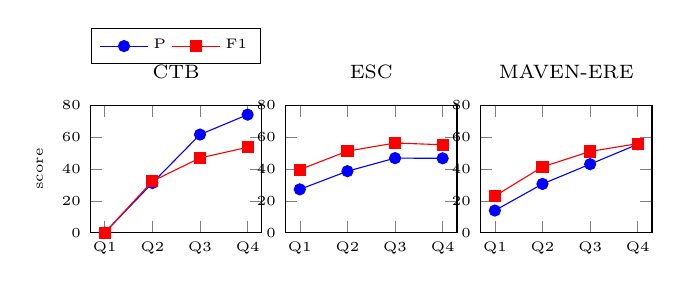
\begin{tikzpicture}
  \begin{groupplot}[
      group style={group size=3 by 1, horizontal sep=3mm},
      width=0.31\linewidth, height=3.2cm,
      ymin=0, ymax=80,
      symbolic x coords={Q1,Q2,Q3,Q4},
      xtick=data,
      tick label style={font=\tiny}, label style={font=\tiny},
      legend style={font=\tiny, at={(0.5,1.32)}, anchor=south, legend columns=2},
    ]
    \nextgroupplot[title={CTB}, title style={font=\scriptsize},
      ylabel={score}, ylabel style={font=\tiny}]
      \addplot[mark=*, blue] coordinates {(Q1,0.0) (Q2,31.2) (Q3,61.6) (Q4,74.1)};
      \addplot[mark=square*, red] coordinates {(Q1,0.0) (Q2,32.3) (Q3,46.9) (Q4,53.6)};
      \legend{P,F1}
    \nextgroupplot[title={ESC}, title style={font=\scriptsize}]
      \addplot[mark=*, blue] coordinates {(Q1,27.2) (Q2,38.6) (Q3,46.8) (Q4,46.7)};
      \addplot[mark=square*, red] coordinates {(Q1,39.6) (Q2,51.2) (Q3,56.3) (Q4,55.2)};
    \nextgroupplot[title={MAVEN-ERE}, title style={font=\scriptsize}]
      \addplot[mark=*, blue] coordinates {(Q1,13.9) (Q2,30.6) (Q3,43.0) (Q4,55.5)};
      \addplot[mark=square*, red] coordinates {(Q1,23.0) (Q2,41.3) (Q3,51.0) (Q4,55.9)};
  \end{groupplot}
  \end{tikzpicture}
  \caption{Precision and F1 by document causal-density quartile (Q1 sparsest --
  Q4 densest), pooled binary-intra, on the three headline runs.}
  \label{fig:density}
\end{figure}

\paragraph{Robustness by backbone.} Documents that exhaust all JSON-parsing
retries are rare but backbone-dependent: 3.3 per run on
\texttt{deepseek-v3.2:nitro} (291 over 87 runs) against 0.1 per run on
\texttt{deepseek-v4-pro} (4 over 38 runs) and 0.6 on the reasoning-tuned
\texttt{qwen3} variant. The v3.2-to-v4-pro backbone upgrade nearly eliminated
parse failures, which also means v3.2-era ablation runs (\S\ref{sec:ablations})
carry a small additional confound, since failed documents score as all-
\textit{norel} (\S\ref{sec:inference}) rather than being excluded.

\paragraph{Causal hallucination is a shared failure mode, not one model's
idiosyncrasy.} A separate cross-backbone analysis of every intra-sentence
prediction logged across the pipeline's candidate backbones (34 qualifying runs
spanning 8 models, filtered to $\mathrm{total\_pairs}>10$ and
$F1_{\text{intra}}>0.30$, predominantly on MAVEN-ERE) asks whether different
backbones fail independently of one another. They do not: on the 1{,}294
intra-sentence pairs scored by more than 5 of the 34 runs, predictions agree far
above chance (Fleiss' $\kappa=0.58$ three-way, $0.70$ binary), 796 of those 1{,}294
pairs (61.5\%) are wrong in \emph{every} covering run regardless of model, and
among the 178 pairs where every covering run unanimously agrees and is wrong,
93\% are phantom causality --- every model inventing a causal link the annotation
says is not there, split almost evenly between the two directions, with
essentially no direction confusion. Every one of the 28 cross-model pairs shows
positive correctness correlation ($\phi$ 0.31--0.65), and majority-vote
ensembling \emph{across models} recovers only 16.2\% accuracy on this hard
subset, barely above the single best model (29.3\%). This is the mirror image of
\S\ref{sec:voting}'s finding: ensembling across demonstration sets works because
per-pass false positives are demonstration-specific and largely independent,
whereas ensembling across backbones does not fix a bias that all of them already
share. It sharpens \citeauthor{gao2023chatgpt}'s (\citeyear{gao2023chatgpt})
original causal-hallucination finding: the failure is not one model's
idiosyncrasy but a property of the task itself, which is precisely what a
document-level, rule-constrained protocol (\S\ref{sec:docprompt}) targets
directly rather than leaving to backbone choice.

\paragraph{False-positive taxonomy.} A keyword-based pass over the false positives
of the three headline runs (searching the text between and around each
mispredicted pair for causal-marker-adjacent cues) shows that reporting verbs
(``said'', ``according to'', ``announced'') appear near 37.3\% of
Causal-TimeBank's 150 binary-intra false positives, 30.0\% of EventStoryLine's
3{,}284, and 5.8\% of MAVEN-ERE's 5{,}862; purely temporal connectives (``after'',
``since'', ``following'') appear near 2.7\%, 8.7\%, and 10.8\% respectively. The
transitive-flattening pattern we originally expected to dominate --- $A \to B \to
C$ read as $A \to C$ --- turns out to be minor: only 1.3--2.8\% of false positives
have a gold $A \to B$ and $B \to C$ edge in the same document (0\% on MAVEN-ERE),
computed exactly from the gold causal graph rather than by keyword search. The
remaining 58--83\% of false positives fit neither pattern under this coarse
heuristic, so most of \method{}'s hallucination is not explained by these two
surface cues alone and needs a proper manual taxonomy; this keyword pass is a
first cut, not a finished analysis.

\paragraph{Qualitative example.} On Causal-TimeBank document
\texttt{APW19980227.0476} (a wire report on a World Court ruling), the model's
sentence-by-sentence reasoning correctly rejects several plausible-looking
non-causal connections --- ``that'' in \emph{`that has blocked the trial'} is
flagged as a relative pronoun, not a causal marker; ``to'' in \emph{`to force the
suspects' extradition'} is flagged as an infinitive of purpose, not an explicit
marker --- and the pass ends with zero predicted causal pairs. The gold
annotation, however, contains exactly the two pairs the model dismissed on those
grounds: the objections \emph{caused} the trial to be blocked, and the Security
Council resolutions \emph{caused} the push for extradition. Both are genuine
causal relations expressed through a purposive or relative-clause construction
rather than an explicit connective like ``because'' or ``therefore''. This is a
concrete instance of the recall cost of the Causal-TimeBank explicit-marker rule
(\S\ref{sec:docprompt}): a rule strict enough to suppress the reporting-verb and
temporal false positives above also suppresses genuine but
non-prototypically-worded causal links, one contributor to Causal-TimeBank's
recall of 39.6 against its precision of 61.1 (Table~\ref{tab:main-results}).

Direction confusion (whether a true positive's predicted direction matches its
gold direction) is out of scope under the binary problem definition adopted in
\S\ref{sec:task}: since we do not evaluate direction, direction errors are not
counted against the metrics we report. For the record, since directed metrics are
also logged, predicted direction disagrees with the stored gold direction on
55.1\% of EventStoryLine's binary true positives, against 1.9\% on MAVEN-ERE and
0.0\% on Causal-TimeBank --- consistent with EventStoryLine's substantially lower
directed (non-collapsed) metrics relative to its binary ones, and a reminder of
why we read binary metrics as primary throughout this paper rather than as a
simplification of a ``truer'' directed number.

% ======================================================================
\section{Conclusion}
\label{sec:conclusion}

We reframed LLM-based Event Causality Identification from per-pair scaffolding to
a single document-level call, guided by a structured reasoning protocol and
explicit coherence rules, and introduced synthetic, decontaminated
chain-of-thought demonstrations: rationalization used at inference time rather
than as fine-tuning data, requiring no human-written rationales, no external
knowledge base, and no model training. The result is a large, precision-driven
gain where causal hallucination is costliest --- +28.1 F1 on Causal-TimeBank,
breaking out of the degenerate high-recall/low-precision regime every LLM baseline
exhibits there --- together with the best precision on MAVEN-ERE and an F1 edge
over the strongest prior LLM method on EventStoryLine. Beyond the headline table,
treating the method's own logged predictions as data to be analyzed, rather than
only as a score to report, surfaced three findings we did not anticipate when
designing the method: majority-vote aggregation over demonstration ensembles is
empirically F1-optimal rather than merely a safe default; precision
\emph{rises}, not falls, with a document's causal density, so sparse documents
rather than dense ones are the real failure mode; and synthetic chain-of-thought
demonstrations help chat-tuned backbones while measurably hurting a
reasoning-tuned one. We take the last of these as evidence that ``more reasoning
in the prompt'' is not a uniformly good design choice, and that scaffold design
should account for what kind of reasoning a backbone already does on its own.

The method is, by construction, a bet on model quality: because it asks the model
to do exactly the kind of long-context, whole-document reasoning that pair-level
scaffolds structurally prevent, we expect it to improve as backbones improve
rather than requiring re-engineering around each new model generation. Our current
evidence for this (\S\ref{sec:scaling}) is directional and single-seed rather than
a controlled crossover result; strengthening it, along with the ablations we
cannot yet support (\S\ref{sec:ablations}), is the paper's main unfinished
business.

% ======================================================================
\section*{Limitations}

\textbf{Comparability.} All \method{} numbers in Table~\ref{tab:main-results} are
computed on the intra-sentence subset of pairs, matching the subset SERE itself
evaluates (\S\ref{sec:task}); this makes the comparison fair rather than
incomplete, but it also means full-document (intra- and inter-sentence)
performance --- a capability the document-level formulation affords precisely
because it does not pay per additional pair --- is not yet measured for any of the
three datasets. Baseline numbers throughout are reproduced from
\citet{hao2026sere} and \citet{cai2025dreci} rather than re-run with our backbone,
and we do not have a same-backbone pair-level control to separate the
document-level formulation's effect from the backbone's; \S\ref{sec:cost} explains
why that control does not currently exist in our pipeline, and reports the
cost-effectiveness argument we use in its place.

\textbf{Evidence maturity.} Several claims in \S\ref{sec:ablations} and
\S\ref{sec:scaling} rest on single-seed or otherwise confounded runs, calibrated
against a measured noise floor of roughly 2--4 F1 on 50-document subsets
(\S\ref{sec:results}); we have tried to flag every such case rather than present
it as settled. Two ablations are currently not just underpowered but structurally
unavailable: isolating decontamination requires a configuration option our
pipeline does not yet expose (it runs unconditionally in both CoT protocols), and
isolating the in-prompt coherence rules requires a controlled comparison we have
not yet run. Our exploratory results on MECI, a multilingual ECI corpus the
pipeline supports, are noisy enough across repeated identical configurations that
we chose not to include them in the main comparison.

\textbf{Method-specific risks.} Decontamination is itself LLM-based, and we have
not conducted a manual audit of generated demonstrations to bound residual
answer-leakage phrasing that survives it. Synthetic CoT generation costs 2--3
extra LLM calls per unique demonstration document (amortized by caching across a
run, but not free), and whether a stronger teacher model can improve the
demonstrations consumed by a weaker or differently-tuned reasoner
(\S\ref{sec:cotbackbone}) remains untested. Long documents with large pair sets
stress the single-call format --- output-length limits, and potentially attention
dilution on the generation side even though we find no such dilution on the
\emph{scoring} side (\S\ref{sec:erroranalysis}) --- and per-document routing or
chunking may be needed at that extreme, though we have not yet characterized where
it starts to bite.

% ======================================================================
% \appendix
% \section{Prompts}
% \begin{itemize}
%   \item Full system/user prompts per dataset (versioned in repo).
%   \item CoT-generation prompts: gold hint, correction hint, decontamination.
%   \item Coherence rule sets per dataset.
% \end{itemize}
% \section{Additional Details}
% \begin{itemize}
%   \item Dataset statistics and label mappings.
%   \item Resampling/tie-breaking details; JSON-repair procedure.
%   \item MECI multilingual results (if not in main text).
% \end{itemize}

% acl.sty already sets \bibliographystyle{acl_natbib} internally.
\bibliography{references}

\end{document}
 